\documentclass[border=2mm]{standalone}
\usepackage{tikz}
\usetikzlibrary{positioning, calc} % Caricato anche calc per calcoli tra coordinate
\usepackage{array} % Per il posizionamento verticale del testo nelle celle

\definecolor{darkred}{rgb}{0.5, 0.0, 0.0}
\definecolor{darkgreen}{rgb}{0.0, 0.5, 0.0}
\definecolor{darkblue}{rgb}{0.0, 0.0, 0.5}

\begin{document}

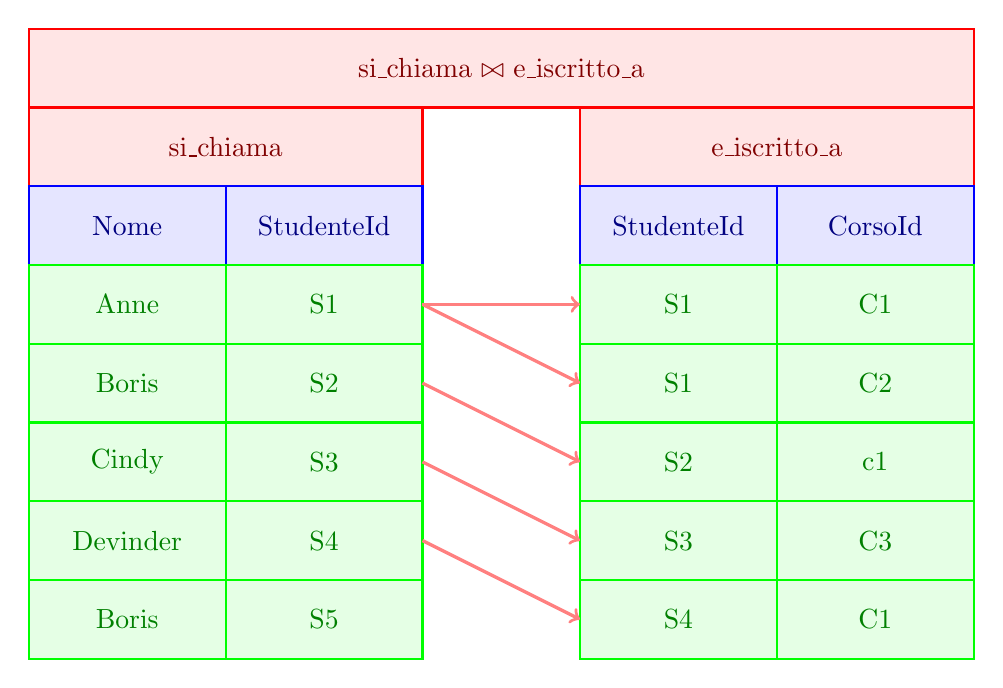
\begin{tikzpicture}
    % Stile per le celle della tabella
    \tikzset{
        table_cell/.style={
            draw=green, % Bordo visibile
            text=darkgreen,
            fill=green!10, % Sfondo
            thick,
            minimum width=2.5cm, % Larghezza minima della cella
            minimum height=1cm, % Altezza minima della cella
            align=center, % Allineamento centrale del testo
            font=\normalsize, % Dimensione del font
            outer sep=0pt, % Rimuove spazio extra intorno al nodo
            inner sep=0.2em % Piccolo spazio interno per il testo
        },
        table_header/.style={
            draw=blue, % Bordo visibile
            text=darkblue,
            fill=blue!10, % Sfondo
            thick,
            minimum width=2.5cm, % Larghezza minima della cella
            minimum height=1cm, % Altezza minima della cella
            align=center, % Allineamento centrale del testo
            font=\normalsize % Dimensione del font
        },
        table_name/.style={
            draw=red, % Bordo visibile
            fill=red!10,
            text=darkred,
            thick,
            minimum width=5cm, % Larghezza minima della cella
            minimum height=1cm, % Altezza minima della cella
            align=center, % Allineamento centrale del testo
            font=\normalsize % Dimensione del font
        }
    }

	\node[table_name,minimum width=12cm] (table_name) at (3.5,1) {si\_chiama $\bowtie$ e\_iscritto\_a};

	\begin{scope}
    % Riga del nome della tabella
    \node[table_name] (t1_table_name) at (0,0) {si\_chiama};

    % Intestazioni
    
    \node[table_header] (t1_header1) at (1.25,-1) {StudenteId};
    \node[table_header] (t1_header2) at (-1.25,-1) {Nome};

    
    % Valori
    \node[table_cell] (t1_row1_col1) at (1.25,-2) {S1};
    \node[table_cell] (t1_row1_col2) at (-1.25,-2) {Anne};

    \node[table_cell] (t1_row2_col1) at (1.25,-3) {S2};
    \node[table_cell] (t1_row2_col2) at (-1.25,-3) {Boris};

    \node[table_cell] (t1_row3_col1) at (1.25,-4) {S3};
    \node[table_cell] (t1_row3_col2) at (-1.25,-4) {Cindy};

    \node[table_cell] (t1_row4_col1) at (1.25,-5) {S4};
    \node[table_cell] (t1_row4_col2) at (-1.25,-5) {Devinder};

    \node[table_cell] (t1_row5_col1) at (1.25,-6) {S5};
    \node[table_cell] (t1_row5_col2) at (-1.25,-6) {Boris};
    \end{scope}
    
    	\begin{scope}[shift={(7,0)}]
    % Riga del nome della tabella
    \node[table_name] (t2_table_name) at (0,0) {e\_iscritto\_a};

    % Intestazioni
    
    \node[table_header] (t2_header1) at (-1.25,-1) {StudenteId};
    \node[table_header] (t2_header2) at (1.25,-1) {CorsoId};

    
    % Valori
    \node[table_cell] (t2_row1_col1) at (-1.25,-2) {S1};
    \node[table_cell] (t2_row1_col2) at (1.25,-2) {C1};

    \node[table_cell] (t2_row2_col1) at (-1.25,-3) {S1};
    \node[table_cell] (t2_row2_col2) at (1.25,-3) {C2};

    \node[table_cell] (t2_row3_col1) at (-1.25,-4) {S2};
    \node[table_cell] (t2_row3_col2) at (1.25,-4) {c1};

    \node[table_cell] (t2_row4_col1) at (-1.25,-5) {S3};
    \node[table_cell] (t2_row4_col2) at (1.25,-5) {C3};

    \node[table_cell] (t2_row5_col1) at (-1.25,-6) {S4};
    \node[table_cell] (t2_row5_col2) at (1.25,-6) {C1};    \end{scope}

    % Collego tutti i S1 della prima tabella a tutti i S1 della seconda
    \draw[red!50, very thick, ->] (t1_row1_col1.east) -- (t2_row1_col1.west);
    \draw[red!50, very thick, ->] (t1_row1_col1.east) -- (t2_row2_col1.west);

    % Collego S2
    \draw[red!50, very thick, ->] (t1_row2_col1.east) -- (t2_row3_col1.west);

    % Collego S3
    \draw[red!50, very thick, ->] (t1_row3_col1.east) -- (t2_row4_col1.west);

    % Collego S4
    \draw[red!50, very thick, ->] (t1_row4_col1.east) -- (t2_row5_col1.west);

    % (S5 non ha corrispondenza nella seconda tabella, quindi non viene collegato)


\end{tikzpicture}
\end{document}
